\documentclass[10pt,twocolumn,letterpaper]{article}
%\usepackage[latin1]{inputenc}

%\usepackage{url}
%\usepackage{booktabs}

\usepackage{iccv}
\usepackage{times}
\usepackage{epsfig}
\usepackage{graphicx}
\usepackage{grffile}
\usepackage{amsmath}
\usepackage{amssymb}
\usepackage{amsmath}
\usepackage{amsfonts}
\usepackage{subfigure}
\usepackage{nonfloat}
\usepackage{url}
%\usepackage[colorlinks=true, linkcolor=green, pagebackref]{hyperref}
\usepackage{textcomp} % for textonehalf
%\usepackage{subfig}
%\usepackage{subref}
%\usepackage{booktabs}

\usepackage{wrapfig}
\graphicspath{{imgs/}{data/renders_turn_table/}{imgs/rendered_results/}{imgs/tabletop_results/}}

\usepackage{xspace}
\renewcommand*{\eg}{e.g.\@\xspace}
\renewcommand*{\ie}{i.e.\@\xspace}
\newcommand*{\ea}{et al.\@\xspace}
\renewcommand*{\vs}{vs.\@\xspace}
%\renewcommand{\arraystretch}{1.5}

%\cvprfinalcopy % *** Uncomment this line for the final submission

\def\iccvPaperID{351} % *** Enter the CVPR Paper ID here
\def\httilde{\mbox{\tt\raisebox{-.5ex}{\symbol{126}}}}

% General notation
\newcommand{\prob}{Pr}
\newcommand{\degree}{^{\circ}}
\newcommand{\feat}{\mathbf{x}}

% Image notation
\newcommand{\rgbdimage}{\mathcal{D}}
\newcommand{\intrinsics}{K}
\newcommand{\pixelidx}{\mathbf{s}}
\newcommand{\edgeimidx}{\mathbf{e}}

% Voxel notation
\newcommand{\voxelgrid}{\mathcal{V}}
\newcommand{\voxel}{v}
\newcommand{\voxidx}{i}
\newcommand{\voxelidxs}{m, n, l}

% Point cloud notation
\newcommand{\project}{\mathbf{p}}
\newcommand{\pcloud}{\mathcal{P}}
\newcommand{\point}{\mathbf{p}}
\newcommand{\normal}{\mathbf{n}}
\newcommand{\updir}{\mathbf{u}}

% Transformations
\newcommand{\trans}{T}
\newcommand{\extrinsics}{H}
\newcommand{\voxelgridtoworld}{\trans_{\voxelgrid \rightarrow w}}


\definecolor{red}{rgb}{0.95,0.4,0.4}
\definecolor{blue}{rgb}{0.4,0.4,0.95}
\definecolor{darkred}{rgb}{0.8,0,0}
\definecolor{darkgreen}{rgb}{0,0.5,0}
\definecolor{grey}{rgb}{0.6,0.6,0.6}

\newcommand{\todo}[1]{\textcolor{red}{TODO: #1}}
\newcommand{\note}[1]{\textcolor{blue}{NOTE: #1}}
\newcommand{\status}[1]{\textcolor{blue}{Status: #1}}
\newcommand{\add}[1]{\textcolor{darkgreen}{#1}}
\newcommand{\remove}[1]{\textcolor{grey}{#1}}

\renewcommand{\paragraph}{\vspace{2pt}\noindent\textbf}

%[citecounter=true, style=ieee]
%\usepackage{biblatex}
%\addbibresource{bibtex/strings.bib}
%\addbibresource{bibtex/main.bib}
%\addbibresource{bibtex/crossrefs.bib}
%addbibresource{\jobname.bib}


\title{Structured Prediction of Unobserved Voxels From a Single Depth Image}

\begin{document}


\maketitle

\begin{abstract}
    %Building a representation of the geometry of a scene is an essential task for many applications including robotic navigation, scene re-lighting and object manipulation.
    %Most existing works to recover the scene geometry rely on combining multiple views of the scene captured from many different directions or use of \emph{a priori} information about the expected semantic make-up of the scene.
Building a complete 3D model of a scene given only a single depth image is underconstrained.
To gain a full volumetric model, one typically needs either multiple views, or a single view together with a library of unambiguous 3D models that will fit the shape of each individual object in the scene.

We hypothesize that objects of dissimilar semantic classes often share similar 3D shape components, enabling a limited dataset to model the shape of a wide range of objects, and hence estimate their hidden geometry.
Demonstrating this hypothesis, we propose an algorithm that can complete the unobserved geometry of table-top-sized objects, based on a supervised model trained on an unrelated dataset of volumetric elements.
Our model maps from a local observation from a single depth image to an estimate of the surface shape in the surrounding neighborhood.
We validate our approach qualitatively and quantitatively on a range of indoor object collections.

\end{abstract}

%%%%%%%%%%%%%%%%%%%%%%%%%%%%%%%%%%%%%%%%%%%%%%%%%%%%%%%%%%%%%%
\section{Introduction}
%\footnote{Potential to add to intro: Psychology: Are humans good at this? Not much evaluation in other work.}
%%%%%%%%%%%%%%%%%%%%%%%%%%%%%%%%%%%%%%%%%%%%%%%%%%%%%%%%%%%%%%


% What is the problem?
We broadly categorize space in our world as being `occupied' and opaque, or `empty' and transparent.
Depth cameras such as the Microsoft Kinect are able to give an estimate of which regions of a scene are composed of free, empty space.
However, each pixel in a depth image only makes an estimate of occupancy in front of the first solid surface encountered along that camera ray.
Occlusion prevents any information from being measured about the occupancy of space beyond that first surface.

% Why is it interesting and important?
There are many applications, however, which critically require a complete representation of the world geometry.
When a robot hand or autonomous vehicle interacts with an unknown object in an unknown environment, a full 3D understanding is required to navigate and prevent collisions.
In photo-editing, the full geometry would enable realistic shadows from a new light source to be automatically added to an image or stereo pair after capture.

% Why is it hard? (E.g., why do naive approaches fail?)
A large amount of computer vision research has been devoted to reconstructing a full 3D world model from RGB or depth images of a scene captured from multiple viewpoints, thus coping with the effects of occlusion  (\eg \cite{seitz2006comparison, izadi-uist-2011}).
Instead, we focus on the task of classifying each voxel in a local 3D scene as being either `occupied' or `empty,' given just a single depth image from one viewpoint.
An example result of our algorithm is displayed in Figure~\ref{fig:intro}.
%% THERE WILL ALWAYS BE HOLES, EVEN WITH KINFU %%

\begin{figure}
     \includegraphics[width=1.0\columnwidth]{banner}
         \caption{\textbf{Our volumetric completion.}
    (a) Intensity image, for illustration only.
    (b) (Input) 3D projection of the depth image, captured from the black arrow's perspective, where occlusions induce large empty spaces.
    (c) Ground truth occupancy.
    (d) (Output) Our {\bf Voxlets} algorithm predicts a plausible completion of the tabletop objects' geometry.}%
    \label{fig:intro}
        \vspace{-10pt}
\end{figure}


%%%%%%%%%%%%%%%%%%%%%%%%%%%%%%%%%%%%%%%%%%%%%%%%%%%%%%%%%%%%%%
%\subsection{Our approach and contributions}
%%%%%%%%%%%%%%%%%%%%%%%%%%%%%%%%%%%%%%%%%%%%%%%%%%%%%%%%%%%%%%

%Given a single depth image, our system predicts whether each voxel in the local scene is occupied by a solid impermeable object, or free and empty.
In effect, we strive to predict the voxelized output of KinectFusion \cite{izadi-uist-2011}, without moving around. %but using only a single depth image of the scene as input instead of multiple views.
We achieve this by learning a mapping from local and semi-regional features on a depth image to a structured prediction of geometry in the region of a query point.
We take inspiration from recent work that segments objects from images using silhouettes learned from different object classes \cite{kim-eccv-2012}.
Their work showed that shape can transcend class categories, enabling shape predictions to be made without the need for semantic understanding.
Because we care about shape, independently of semantic understanding, we are free to use training objects that differ from the objects present in the test scene.

The key contributions that underpin our novel depth image to voxel geometry framework are:

\noindent i) \emph{Voxlets}: a representation of local multi-voxel geometry.
We use a structured Random Forest to learn a mapping from a point in a depth image to a structured prediction of the geometry in the region around that point.

%\noindent ii) \emph{Features}: we demonstrate the efficacy of a feature representation taken directly from a signed distance field.
%This representation allows us to efficiently find the correlation between occluded geometry and observed depth measurements.

\noindent ii) \emph{Fitted predictions}: as opposed to naively placing voxlets directly into a scene, we demonstrate the efficacy of selecting the best ones based on their fit to the observed geometry.

\noindent iii) \emph{Datasets}: we introduce both synthetic and real world datasets, setting a new standard for evaluating volumetric completion algorithms.
The real dataset contains $90$ scans of different object configurations.




\begin{figure*}
     \includegraphics[width=\linewidth]{alg_overview}
         \caption{\textbf{2D overview of our algorithm.}
    (a) We model the world as a grid of voxels representing the signed distance to the nearest surface.
    Here, we show an overhead view of a scene featuring two objects.
    (b) When observed by a depth camera, only the first voxel along each ray is seen.
    This leaves a region of unknown occupancy extending beyond the depth surface.
    At test time, we define a cuboid region of voxels, $\mathcal{R}$, around each query point, $\pixelidx$, aligned with the normal at $\pixelidx$.
    (c) Our structured Random Forest makes a prediction for the signed distance of each of the voxels in $\mathcal{R}$ given a feature $\mathbf{x}(\mathbf{s})$ computed from the observed geometry.
    (d) This prediction is placed into the scene, and used to update the values of the voxels.
    (e) The aggregation of multiple such predictions forms our final occupancy estimate.}%
    \label{fig:overview}
    \vspace{-6pt}
\end{figure*}



%\begin{figure}[!t]
%    \centering
%    \subfigure[Voxel world model]{%
%        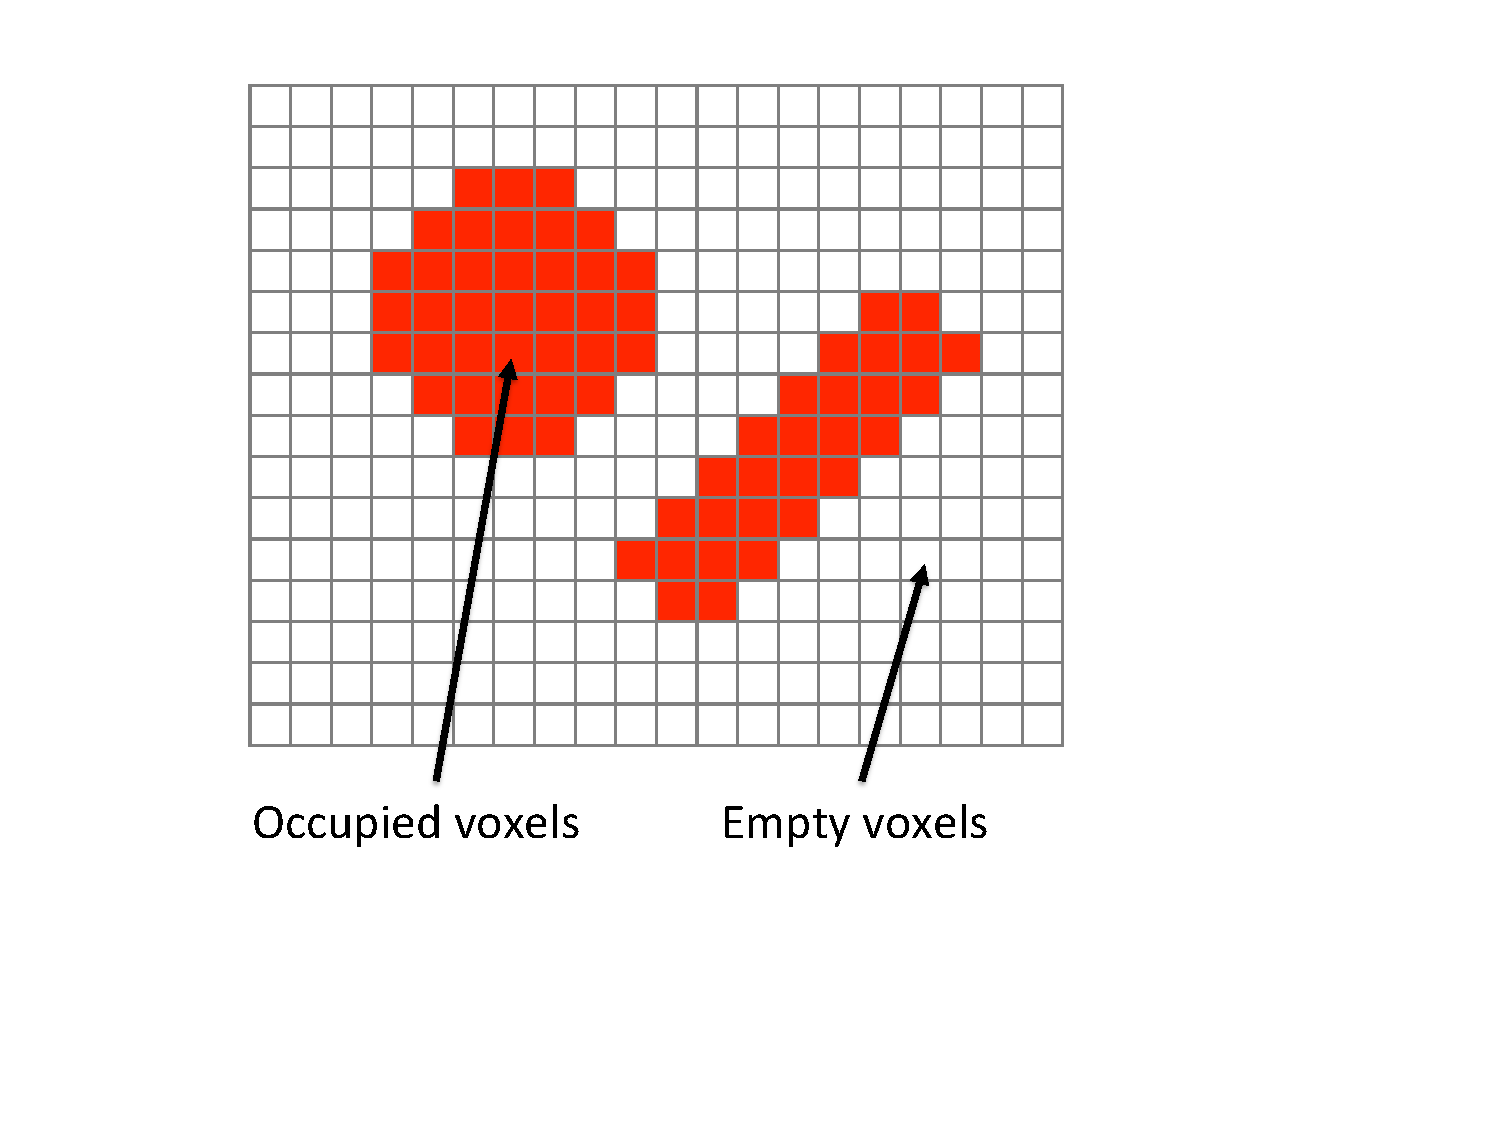
\includegraphics[width=0.48\columnwidth, clip=true, trim=110 105 205 30]{fig_1}}
%        \hfill
%    \subfigure[Depth rendering of world]{%
%        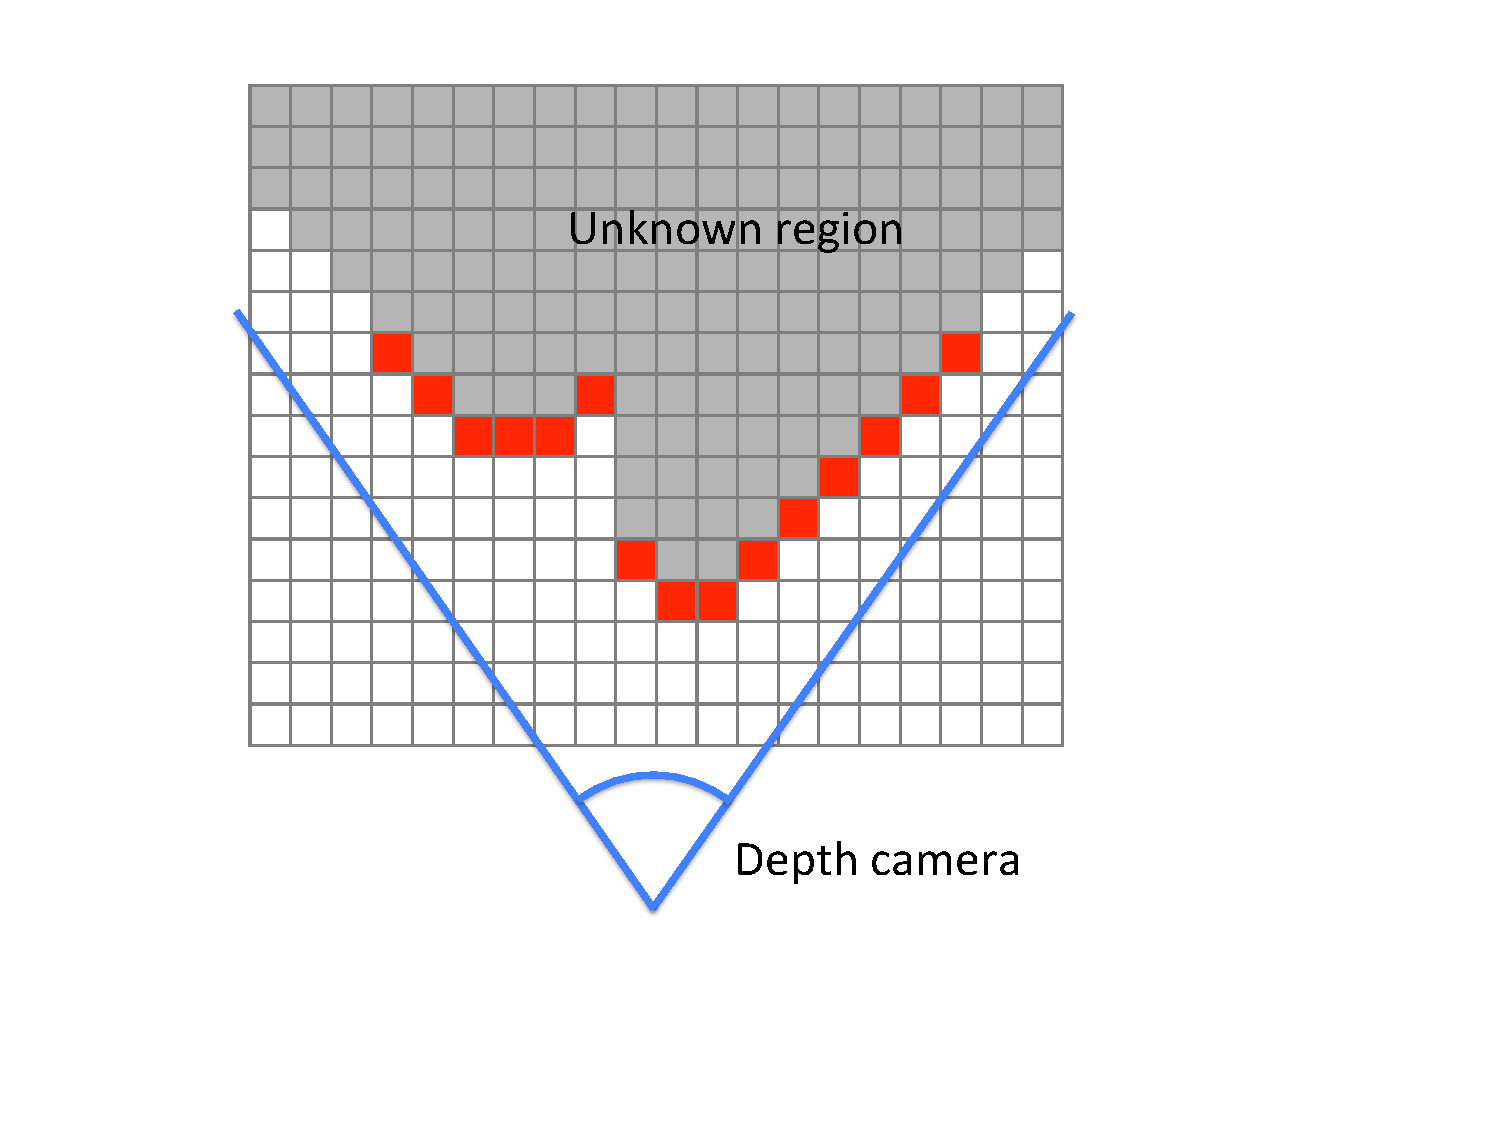
\includegraphics[width=0.48\columnwidth, clip=true, trim=110 105 205 30]{fig_1b}}
%    \caption{
%    We model our world as a grid of voxels, each of which is either occupied or empty (vacant).
%    An overhead view of a coarse 2D representation of this is shown in (a).
%    When observed by a depth camera, only the first voxel along each ray is seen.
%    This leaves a region of unknown occupancy extending beyond the depth surface (b).
%    The aim of our algorithm is to predict the state of the voxels in this unknown region.}%
%    \label{fig:intro}
%\end{figure}



%%%%%%%%%%%%%%%%%%%%%%%%%%%%%%%%%%%%%%%%%%%%%%%%%%%%%%%%%%%%%%
\section{Related work}
%%%%%%%%%%%%%%%%%%%%%%%%%%%%%%%%%%%%%%%%%%%%%%%%%%%%%%%%%%%%%%

%Most prior work in the area of completing missing data can be categorized according to its application domain (\eg meshes \cite{schnabel-eurographics-2009, ju-cst-2009}, 2D images \cite{gupta-cvpr-2011} or depth images \cite{shen-tog-2012}).


%\subsection{Taxonomy of related works}
Here we review related methods for completing unknown regions of visual data.
While similar, we do not cover the problem of 2D image completion.
Work in 2D completion usually relies on the availability of extremely large numbers of similar images~\cite{hays-siggraph-2007}, or on the assumption that the necessary structure for completion is present in the input data~\cite{criminisi-cvpr-2003}.
Image completion typically aims for a visually plausible output, as opposed to accurate approximation of ground truth.
Additionally, our approach utilizes standard consumer hardware, so we do not review work that requires highly specialized equipment~\cite{velten-nature-2012}.


%%%%%%%%%%%%%%%%%%%%%%%%%%%%%%%%%%%%%%%%
\paragraph{3D primitives}\newline
`Geons' were proposed by \cite{bieberman-rbc-1987} as a set of 3D primitives, such as cylinders and cuboids, used by humans in their recognition of object shapes.
While in theory, geons could be used by computers as building blocks to describe natural objects, in practice, this was found to be challenging \cite{dickinson-iavc-1997} due to their ``idealized nature'', requirement for part segmentation, labeling errors, and the coarseness of features used to extract geons in the first place.
%Besl - hand-defined
However, fitting bounding boxes has recently become a popular method to explain the arrangement of objects in a scene.
Recent work has successfully incorporated high-level information such as gravity and stability
 \cite{shao-siggraphasia-2014, jia-pami-2015}, and made use of training data to accurately detect bounding box locations \cite{hedau-cvpr-2012}.
%Shao \ea \cite{shao-siggraphasia-2014} manual provided
Gupta \ea \cite{gupta-cvpr-2011} estimate voxel occupancy from a 2D image, which is regularized using cuboid bounding box hypotheses.
The obvious problem with bounding box style methods is that they can only give coarse shape information, which is ill suited for geometry completion.
%\todo{Wasn't one+ of these dependent on human initialization of some form? If so, say that.}

Our work, also makes use of 3D primitives.
However, unlike geons which are fixed in shape, we learn a flexible distribution of shapes from training data.
We are also able to make more fine-grained predictions than bounding boxes.


%%%%%%%%%%%%%%%%%%%%%%%%%%%%%%%%%%%%%%%%
\paragraph{Specific shape models}\newline
If prior knowledge is available about the objects present in the scene, in the form of 3D models, then an instance-level model can be fitted to the observed depths.
This gives a good recovery of missing geometry of that object \cite{hinterstoisser-accv-2012, drost-3dimpvt-2012,brachmann2014learning}.
Some works focus on the broader problem where an exact match is not present in the training set.
Shen~\ea~\cite{shen-tog-2012} complete the missing regions of a single object using an assembly of parts from several different models in a CAD database.
Cocias \ea \cite{cocias-cgvcv-2013} directly deform a mesh to fit to a point cloud, while Prisacariu and Reid \cite{prisacariu-iccv-2011} fit a class-level manifold model to the image data.
%\note{Cite 3D ShapeNets CVPR 2015}

%Collecting training data for this is laborious and costly, and currently there do not exist enough 3D models suitable for accurately completing most real-world scenes.
All these methods, however, rely on the availability of some form of specific prior model, and on accurate detection to localize each object of interest in the scene.
In our approach, we set out to get as much shape information as possible \emph{without semantics}, thus remaining free of its associated machinery and limitations.


%%%%%%%%%%%%%%%%%%%%%%%%%%%%%%%%%%%%%%%%
\paragraph{Surface completion}\newline
Silberman \ea \cite{silberman-eccv-2014} tackle the completion of an incomplete multi-view reconstruction as a 2D surface completion problem.
By detecting planes, they can complete their contours in a 2D projection using a novel CRF method.
That method, however, assumes a piecewise-planar scene, and requires multiple views as input.
Davis \ea \cite{davis-3dpvt-2002} complete surfaces by operating directly on the \emph{signed distance field}, the zero level-set of which defines the surface location. They diffuse the signed distance field across holes in the mesh to fill in the gaps.
\cite{harary-tog-2013} use a data-driven approach, finding matches in the mesh to fill the missing region.
Symmetry can be leveraged to complete some types of objects, \eg \cite{law-cviu-2010, thrun-iccv-2005, kroemer-humanoids-2012}.
However, this can be brittle, and if symmetry cannot be detected at all, then no prediction can be made.

All of these completion methods are only suitable where the set of missing data is small relative to the size of the observed data.
In our case, we are completing significant geometry of an unknown volume, which is typically at least as large as the observed fragments.


%%%%%%%%%%%%%%%%%%%%%%%%%%%%%%%%%%%%%%%%
\paragraph{Voxel space reasoning}\newline
Finally, the two algorithms most similar to ours both make predictions of full scene geometry from a single depth image.
Kim \ea \cite{kim-iccv-2013} use a CRF model over a voxel representation of a scene to simultaneously predict occupancy, visibility, and semantic labeling of voxels from an RGBD image.
For training, they use manually labeled top-down views of the scene.
They model the probability of a voxel being occupied as a Gaussian centered on the first observed voxel along a camera ray.
However, high-order-terms in the CRF are used to enforce planar structures and for `objects' to remain contiguous.
Unlike \cite{kim-iccv-2013}, our algorithm does not require any semantic or appearance information.

Similarly,  Zheng \ea \cite{zheng-cvpr-2013} go from a single depth image to a voxel representation of a scene.
Their core algorithm consists of two parts.
First, they complete missing voxels by extruding visible points in the detected Manhattan World directions of the scene.
This is related to the completion method of \cite{kroemer-humanoids-2012}.
Secondly, they use physics-based reasoning to fill in missing data to ensure connectedness and stability.
The physics-based reasoning is clearly useful, for example, where supporting object parts may be occluded.
While we compare against a version of this baseline, such voxel completion by extrusion is limited to Manhattan World propagation of the observed volume.

In contrast to these rule-based methods, we make \emph{structured} predictions in 3D space, and reason about shape variation using models learned from 3D training data.
%we are able to complete objects where the points making up the objects are hard to see.}


%%%%%%%%%%%%%%%%%%%%%%%%%%%%%%%%%%%%%%%%
\paragraph{Depth datasets}\newline
While large datasets such as NYU-Depth V2 \cite{silberman-eccv-2012} and the recently introduced SUN RGB-D dataset \cite{SUNRGBD} exist for single depth images, few datasets are available containing full 3D reconstructions.
At an object level, datasets exist that capture the full $360^{\circ}$ shape of individual objects using turntables.
The Washington RGBD Object dataset \cite{lai2011large, lai2014unsupervised} contains hundreds of individual objects, but without detailed camera poses, making reconstruction difficult.
The Bigbird dataset~\cite{singh-icra-2014} is comprised of household objects along with ground truth camera poses and registered meshes.
At a scene level, the small number of datasets featuring full reconstructions tend to have a limited number of examples~\eg \cite{shotton2013scene}.

In this work, we introduce a new dataset consisting of $90$ different configurations of real objects, captured in tabletop scenarios, complete with full 3D reconstructions.



%%%%%%%%%%%%%%%%%%%%



% %%%%%%%%%%%%%%%%%%%%%%%%%%%%%%%%%%%%%%%%%%%%%%%%%%%%%%%%%%%%%%%%%%%%%%%%%%%%%%%%
\section{Voxlets algorithm overview}
% %%%%%%%%%%%%%%%%%%%%%%%%%%%%%%%%%%%%%%%%%%%%%%%%%%%%%%%%%%%%%%%%%%%%%%%%%%%%%%%%


\newcommand{\voxregion}{\mathcal{R}}

We model the geometry around an object as a regular grid of voxels $\voxelgrid = \{\voxel_\voxidx\}$.
Following works such as \cite{curless1996volumetric, izadi-uist-2011, prisacariu-iccv-2011}, each $\voxel_\voxidx \in [-d_{\max}, d_{\max}]$ denotes the Truncated Signed Distance Function (TSDF) of the volume, where the zero level-set of $\voxelgrid$ represents a surface.
Each voxel, $\voxel_\voxidx$, stores the distance to the nearest surface, truncated to a maximum value of $d_{\max}$.
Here, $\voxel_\voxidx$ is negative if voxel $\voxidx$ is inside solid opaque matter, and positive if it is in free space.
Our algorithm maps a 3D point, $\pixelidx$, from the observed depth image, $\rgbdimage$, to a prediction of the TSDF in a voxel neighborhood about that point.
The aggregation of such predictions for multiple points on the input gives our final TSDF prediction for the scene.
A 2D overview of our approach is depicted in Figure~\ref{fig:overview}.

%$\project(\pixelidx)$, where $\project(\pixelidx)$ is the 3D location of $\pixelidx$ in world space.

%\paragraph{Voxel grid alignment}
%We make our predictions in a voxel grid aligned with world coordinates.
%In practice this means that the z direction of the voxel grid is aligned with the up direction of the world space.
%We do not make any Manhattan World assumptions so are free to position the voxel grid at any orientation about the z-axis.


\paragraph{Support regions}\newline
The support region $\voxregion \subset \voxelgrid$ is a set of voxels in the neighborhood of $\pixelidx$, for which our model can make a prediction of the TSDF.
Each $\voxregion$ is a fixed-size cuboid of voxels, whose x-axis is aligned with the measured normal direction %relative to the camera
at $\pixelidx$ (Figure \ref{fig:overview} (b)).
The size of $\voxregion$ is defined so that it is large enough to capture local occupancy information at an object level, but not so large that it would span the entire scene.
In a 2D world, the location of $\pixelidx$ and the direction of its normal can unambiguously define the location and orientation of $\voxregion$.
In 3D however, there is an unconstrained degree of freedom, namely rotation of the cuboid about the axis of the normal.
We resolve this by aligning the cuboid such that its z direction is coincident with the world z-axis, \ie the `up' direction of the scene.
The top and bottom face of each cuboid region $\voxregion$ is therefore parallel with the world's automatically detected ground plane.

%The normal at $\pixelidx$ is used to constrain the degree of freedom around the z-axis.
%\todo{Figure for this!}
%The cuboid is then rotated about the z-axis so that its y-axis is perpendicular to the normal at $\project(\pixelidx)$.

\paragraph{Voxlets}\newline
At test time, we extract a feature description for $\voxregion$ from the observed geometry.
Building a structured Random Forest \cite{dollar-iccv-2013}, we can make a prediction of the full, occluded, geometry inside of $\voxregion$.
We call this prediction of geometry a \emph{voxlet}.
The voxlet, which comes out of the forest in canonical alignment, is then transformed from its local coordinate system into world space to fill the voxels in $\voxregion$ (Figure \ref{fig:overview} (d)).
The accumulation of multiple such predictions forms our final prediction of the full TSDF.

%This transformation is the rotation $\Lambda$ followed by the translation $\mathbf{p}(\mathbf{\pixelidx}) - C(\mathcal{S})$, where $\mathbf{p}(\mathbf{\pixelidx})$ is the projection of $\pixelidx$ into world space, and $C(\mathcal{S})$ is the center of the voxlet.
%\note{This notation and explanation is a bit of a mess --- suggestions welcome! Also need to reference the figure in the text. Figure will ultimately be split into (a), (b) etc to make this easier.}


%\paragraph{Training}
%At training time, we similarly define a region $\voxregion$ around each point $\pixelidx$, again of a fixed size.
%To help make our algorithm robust to different arrangements of objects we separate our ground truth grid into regions, and only extract ground truth voxels from the region associated with the point $\pixelidx$.
%In this case, the ground truth values of $\voxelgrid$ and hence $\voxregion$ are known.
%We use these ground truth TSDF values, together with the ground truth representations, to train a Random Forest, as explained in  Section \ref{sec:forest_train}.



%The Random Forest--based model weights feature space to make structured predictions of the truncated signed distance function in the surrounding region.


% %%%%%%%%%%%%%%%%%%%%%%%%%%%%%%%%%%%%%%%%%%%%%%%%%%%%%%%%%%%%%%%%%%%%%%%%%%%%%%%%
\section{Learning a mapping from features to voxlets}
\label{sec:forest_train}
% %%%%%%%%%%%%%%%%%%%%%%%%%%%%%%%%%%%%%%%%%%%%%%%%%%%%%%%%%%%%%%%%%%%%%%%%%%%%%%%%
We pose unobserved geometry estimation, given partial observed information, as a supervised learning problem.
More specifically, our goal is to learn a function $f: \mathcal{X}\to \mathcal{Y}$, that maps a feature vector $\mathbf{x} \in \mathcal{X}$, computed from observed geometry, to the output space $\mathbf{y} \in \mathcal{Y}$ representing the corresponding 3D geometry in the region $\mathcal{R}$ around $\mathbf{x}$.
Unlike standard classification, where the goal is to predict a category label for each $\mathbf{x}$, our output space is a multi-dimensional vector $\mathbf{y} \in \mathbb{R}^{w\times{}d\times{}h}$ that encodes the TSDF values in the local region.
The dimensionality of $\mathbf{y}$ is prohibitively large, making it difficult to use standard multivariate regression approaches, \eg \cite{criminisi2013decision}.
Inspired by the recent work of Doll{\'a}r and Zitnick~\cite{dollar-iccv-2013}, we use a structured Random Forest to learn the function $f$.

\subsection{Training}
Our training set, $\left\{(\mathbf{x}_1, \mathbf{y}_1), ..., (\mathbf{x}_n, \mathbf{y}_n)\right\}$, is comprised of regions sampled from full 3D reconstructions captured $360^{\circ}$ around each scene.
To train the structured forest, we pass a bagged subset of the training set to each tree, starting at the root node.
% subset of the training set to each node in the tree, starting at the root.
Each node is then tasked with splitting the data so that the $\mathbf{x}$'s sent to its children are as similar as possible in shape, \ie with similar $\mathbf{y}$'s.
Instead of minimizing the structured loss directly, \cite{dollar-iccv-2013} approximates this loss at each node using a classification loss.
To convert the structured problem into a classification one, we temporarily create two classes by clustering: Before splitting the data at a node, we sample a different random subset of the dimensions of each $\mathbf{v}_i$, reduce their dimensionality to $M$ dimensions, and then cluster.
Then a standard classification loss can be used on this new discretization, to evaluate the quality of different candidate splits for each $\mathbf{x}_i$.
In practice, we efficiently perform this dimensionality reduction and clustering at each node using randomized PCA~\cite{halko-siam-2011}.
A training example is then assigned to one of the two possible clusters $K$ based on the sign of the values of its first principal component.
This process is repeated until we cannot split the data any further.
Finally, as in \cite{dollar-iccv-2013}, each leaf node stores the medoid of all the examples that have arrived there, which we refer to as a \emph{voxlet}.
We store the medoid for efficiency reasons but it is also possible to store multiple modes, \eg~\cite{girshick2011efficient}.


\subsection{Features}
\begin{wrapfigure}[8]{r}{0.36\columnwidth}
  \vspace{-18pt}
  \centering
    \includegraphics[width=0.36\columnwidth, clip=true, trim=130 210 340 80, page=9]{spider_cobweb}
    \vspace{-12pt}
  \caption{Offset feature.}%The offset feature}
      \vspace{-8pt}
    \label{fig:offset_feature}
\end{wrapfigure}
Our feature descriptor $\mathbf{x}$ consists of simple pairwise distance comparisons of the input depth image $\rgbdimage$.
We do not use appearance information, instead favoring shape cues provided by the depth image.
These offset features are fast to compute, and capture the surface shape in the immediate neighborhood of a point $\pixelidx$ \cite{shotton-cvpr-2011}.
Each dimension, $x_\text{off}$, computes the difference between the depth from the camera at $\pixelidx$'s pixel and the depth at a predetermined offset $\Delta$ (Figure \ref{fig:offset_feature}). We define
\begin{align}
x_\text{off} (\pixelidx, \psi, t) &= \rgbdimage(\pixelidx) - \rgbdimage(\pixelidx + \Delta), \, \text{where} \\
\Delta &= M(t) (\sin(\psi), \cos(\psi)).
\end{align}
Here $M(t) = (t\cdotp f_c)/\rgbdimage(\pixelidx)$ uses the focal length $f_c$ to map a distance in world space to a pixel offset.
For a single point $\pixelidx$, we compute $x_\text{off} (\pixelidx, \psi, t)$ for a range of different values of $\psi$ and $t$, and concatenate the results into a feature vector $\feat$.
For our experiments we use $\psi, \,\, t \in \{0\degree, 45\degree, \ldots, 315\degree\} \times \{0.01m, 0.02m, \hdots 0.10m\}$, where $m$ is meters, resulting in an 80-dimensional feature.
%\note{Mention we pre-compute x offline?}


\paragraph{Pre-segmentation for clutter}\newline
Real world scenes contain clutter and interacting objects.
This poses a challenge when we are extracting our training regions.
While it is possible to represent the shape variation of isolated objects, modeling variations in arrangements of objects is much harder.
This is intuitive, as the space of geometry induced by object combinations is much larger than that of individual objects.
To overcome this problem, we perform an unsupervised segmentation of the \emph{training} scenes, to separate individual objects.
At training time, we assign a label, obtained from connected components, to each occupied voxel ($\voxel_i \textless 0$) in $\voxelgrid$, such that voxels with the same label are well connected to each other, and voxels with different labels are separated by some amount of free space.
When extracting a training region $\voxregion$, from $\voxelgrid$, we note the label at $\pixelidx$, and only voxels with the same label are included in the region.
For an example of this segmentation see Figure~\ref{fig:method_details} (b).
This encourages each training region to only model the shape of isolated objects.
If objects are not well segmented at this stage, it is not a problem, but that node will likely make conjoined predictions at test time.

\section{Predicting occupancy at test time}
Each tree in our forest makes a prediction about how the volume surrounding a point in the input depth image is occupied. Our trees perform inference very efficiently, but in practice, it is unnecessary to make a prediction densely for every location in the input, because closely neighboring locations tend to yield similar predictions.
We ignore locations where the normal points away from the camera, and also reject locations that point upward (as defined by the scene's `up' direction).
We then sample locations throughout the input image, spanning the spectrum of depths, to ensure uniform scene coverage. We only predict occupancy for regions about these locations (dots in Figure~\ref{fig:method_details} (c)).
For this set of locations, we simply traverse a tree down to a leaf node, and return the voxlet stored there in training (Figure~\ref{fig:overview} (c)).
In Figure~\ref{fig:voxlets}, we illustrate a few voxlets and their world positions, predicted for a real scene.

\begin{figure}[t]
     \includegraphics[width=1.0\columnwidth]{imgs/method_details.png}
         \caption{(a) RGB image, not used in our algorithm. (b) Automatic pre-segmentation of full geometry, performed if this were a training image. (c) Sample locations, shown as red dots, where occupancy predictions are made for a test depth image.}
    \label{fig:method_details}
    \vspace{-6pt}
\end{figure}

\subsection{Choosing the best prediction}
\label{sec:agg_predictions}
Each leaf node in each tree in our forest stores a voxlet, \ie the medoid of the examples that landed at that node.
For a given location in the input depth image, each tree will vote for a non-unique voxlet.
We investigated three strategies to combine these region predictions from the different trees:

\noindent\textbf{Forest Mean} We simply take the mean of the voxlets as the forest prediction.
We note that the truncation of the signed distance function helps to make this style of accumulation robust.
A single incorrect estimation at a voxel can only be wrong by a maximum amount of $2d_{\max}$, where $d_{\max}$ is the level at which the distance function is truncated.

\noindent\textbf{Forest Medoid} The previous approach can produce artifacts as a result of the averaging.
Selecting the medoid voxlet of all of the trees (\ie the medoid of the medoids) gives more robustness to outliers.

\noindent\textbf{Observed Fit} Neither of the previous two approaches forces predicted voxlets to be consistent with the partially observed geometry from the input depth image $\rgbdimage$.
To achieve this consistency, we first compute an observed TSDF for $\rgbdimage$.
We then select the voxlet, from the set of forest proposals, that best matches in the narrow band of the observed TSDF, \ie that which has the lowest sum of squared error across the voxels in the narrow band.

These alternatives are evaluated in Section \ref{sec:exp_tt}.
For the final prediction of the output TSDF grid $\voxelgrid$, regardless of strategy, we average the predictions of the overlapping voxlets (Figure \ref{fig:overview} (e)).
If a voxel in $\voxelgrid$ has no predictions made for it, we mark it as empty (\ie $d_{\max}$).
Marching cubes \cite{lorensen-siggraph-2013}, or its variants, can be used to convert the final predicted TSDF to a mesh by finding the level-set of zero.


\subsection{Implementation details}
Given the large dimensionality of ouptput space $\mathcal{Y}$, equal to the size of the support region $\mathcal{R}$, we perform an initial dimensionality reduction using PCA to 400 dimensions.
Due to the large amount of redundancy in each region sample, we empirically found this to have little impact on the quality of our results, yet it provides a large speed up at training time, and reduces storage requirements.
We use an ensemble of $40$ trees with simple axis aligned feature tests at each node, that are grown until there is a minimum of 5 examples at a node, up to a maximum of depth 14.
When clustering the data at each node, we set the subset of random dimensions, $M$, for the randomized PCA to $20$.
At test time, we only make predictions for 300 locations in the input depth image, sampling each point with a probability proportional to its depth.
We truncate the TSDF at $d_{max} = |d_{min}| = 0.02m$.

In our experiments, we predict one of two different size voxlets (requiring two different forests).
The first voxlet is centered at $\pixelidx$ and is longer in the y-direction ($0.15m \times 0.3m \times 0.15m$).
This is the direction that is approximately parallel to the normal at $\pixelidx$ (Figure \ref{fig:overview} (b)).
This allows the voxlet to make a larger prediction \emph{backwards} into the scene, compared to \emph{sideways} which typically already has observed data.
The second voxlet is taller ($0.15m \times 0.3m \times 0.375m$) and its base is fixed to the ground plane.
It is more suitable for making predictions for semi occluded geometry.
For a given sample location in a depth image at test time, we randomly choose one of the two forests to make a prediction.
We will release our code and datasets with this paper, to ease future comparisons.
%For our experiments, we smooth the noisy Kinect depth data using bilateral filtering.
%We then detect the largest approximately horizontal plane in the reprojected 3D points, and use this to estimate the `up' direction of the scene.
%Our voxel grid $\voxelgrid$ lies on top of this predicted plane.\note{OMA: do we still do this?}


%\newcommand{\voxletsubwidth}{0.41\columnwidth}
%\begin{figure}
%     \includegraphics[width=0.32\columnwidth, clip=true, trim=110 30 110 30]{voxlets/pca_render_1.png}
%     \includegraphics[width=0.32\columnwidth, clip=true, trim=110 30 110 30]{voxlets/pca_render_4.png}
%     \includegraphics[width=0.32\columnwidth, clip=true, trim=110 30 110 30]{voxlets/pca_render_8.png} \\
%     \includegraphics[width=0.32\columnwidth, clip=true, trim=110 30 110 30]{voxlets/pca_render_9.png}
%     \includegraphics[width=0.32\columnwidth, clip=true, trim=110 30 110 30]{voxlets/pca_render_16.png}
%     \includegraphics[width=0.32\columnwidth, clip=true, trim=110 30 110 30]{voxlets/pca_render_46.png}
%     \caption{Some exemplar training voxlets extracted from the synthetic dataset in Section \ref{sec:datasets}.
%     Each voxlet can be seen to capture a section of the geometry of the scene. \textcolor{red}{TMP FIG, and explain this surface visualization, vs voxlets which are volume-occupancy.}}
%     \label{fig:voxlets}
%\end{figure}
\begin{figure}[t]
     \includegraphics[width=1.0\columnwidth]{imgs/scene_voxlets}
         \caption{Each tree predicts the occupancy at each sample location, in the form of a voxlet, shown for the scene in Figure~\ref{fig:method_details}. Here we depict just three voxlets that have been meshed using marching cubes, but hundreds of predictions are made in practice.}
    \label{fig:voxlets}
    \vspace{-6pt}
\end{figure}




%%%%%%%%%%%%%%%%%%%%%%%%%%%%%%%%%%%%%%%%%%%%%%%%%%%%%%%%%%%%%%%%%%%%%%%%%%%%%%%%
\section{Datasets}
%%%%%%%%%%%%%%%%%%%%%%%%%%%%%%%%%%%%%%%%%%%%%%%%%%%%%%%%%%%%%%%%%%%%%%%%%%%%%%%%
\label{sec:datasets}
Existing RGBD datasets of real scenes were typically captured to evaluate semantic segmentation, object detection, or camera pose estimation.
To our knowledge, there are no standard datasets that capture the full geometry of a large number of scenes, without sections of missing data caused by occlusion.
To overcome this problem, we introduce two new tabletop-object datasets, that we will make available to aid benchmarking of volumetric completion.
Sample scenes from both datasets can be seen in Figures~\ref{fig:synth_results} and \ref{fig:tabletop_res}.

% \paragraph{Synthetic dataset D1}
Our \textbf{synthetic} dataset consists of 500 `scenes', each featuring a random arrangement of between 4 and 10 3D primitives from a set of 20.
These random, but physically plausible, arrangements were formed by dropping objects onto a plane using a physics simulator.
The ground truth TSDF is computed by fusing together the depth images from 42 cameras on a hemisphere viewing each scene.
This dataset allows us to easily demonstrate and quantify the effects of various parts of our algorithm in the absence of real world sensor noise.
For testing, we perform a 60/40 train/test split at a scene level, and randomly select one of the 42 input views for reconstructing.
%At test time, one image is selected from the 42 input images for a test scene and reconstruction performed.

%\paragraph{Desks dataset D2}
Our \textbf{tabletop} dataset contains the full geometry of 90 configurations of real objects, reconstructed using the Kinect Fusion implementation of \cite{2014arXiv1410.0925P}.
This is seven times larger than the volumetric dataset used in~\cite{zheng-cvpr-2013}, which was not available for experiments.
Each scene is composed of between 2 to 6 household objects from a set of 50, placed on a tabletop.
We manually annotated the extents of the test volume for each scene.
Predictions outside this domain are not used during evaluation.
The dataset is split into 60 training and 30 testing scenes, captured in two different locations, where the objects do not overlap across the split.
We include the raw color and depth frames, together with the reconstructed mesh for each scene.
It is worth noting that this ground truth datatset is only accurate up to the reconstruction error of~\cite{2014arXiv1410.0925P}.



%%%%%%%%%%%%%%%%%%%%%%%%%%%%%%%%%%%%%%%%%%%%%%%%%%%%%%%%%%%%%%%%%%%%%%%%%%%%%%%%
\section{Experiments}
%%%%%%%%%%%%%%%%%%%%%%%%%%%%%%%%%%%%%%%%%%%%%%%%%%%%%%%%%%%%%%%%%%%%%%%%%%%%%%%%
We evaluate our {\bf Voxlets} approach using four different datasets.
The ultimate aim of our algorithm is to accurately classify free space around objects in indoor scenes.
Therefore, we report the per-voxel precision and recall over all the test data, using the sign of the accumulated TSDF as the final binary prediction of occupancy.
We additionally report the Intersection over Union (IoU) of the predicted occupancy, compared to the ground truth.

To quantitatively evaluate our method, we use the manually defined testing volumes for each dataset and make predictions within these regions.
The `up' direction is found from the ground plane of this volume.
For real world usage, this plane and its orientation could be automatically detected~\cite{silberman-eccv-2012}.

%In our work, we manually annotate the ground plane and the region on the plane in which we wish to make a prediction of geometry.
%
%To find our test volume, we find the minimum volume axis-aligned bounding box for the ground truth voxel data before padding this voxel grid with 10cm of padding in each axis direction.


%%%%%%%%%%%%%%%%%%%%%%%%%%%%%%%%%%%%%%%%%%%%
\subsection{Single objects}
First we evaluate our method on the BigBIRD single object turntable dataset \cite{singh-icra-2014}.
We compare our {\bf Voxlets} algorithm to two other baselines: a bounding box approach and the method of Zheng \ea \cite{zheng-cvpr-2013}.
For the bounding box baseline, we fit a minimum-area bounding box to the 3D points belonging to the object, as defined by the ground truth object segmentation mask provided by \cite{singh-icra-2014}.
We are careful to remove points with normals perpendicular to the viewing direction, as these `flying pixels' can have a large adverse effect on bounding box predictions.
All voxels inside the bounding box are assumed to be occupied, while those outside are labeled as empty.
Since we use the ground truth mask to fit the box, this can be viewed as the best possible bounding box, given the observed data.
For the comparison to Zheng~\ea~\cite{zheng-cvpr-2013}, we use the algorithm for reconstructing voxel occupancy as described in Section 2 of their paper.
We find the Manhattan axes of the scene from the minimum area bounding box aligned with the ground truth voxel grid.
We then perform their axis-aligned voxel search for each unobserved voxel, marking voxels as ‘filled’ if more than two Manhattan directions hit a voxel directly observed by the camera.
As this is a single object evaluation, we do not use the extra physical reasoning step.

The results from this quantitative analysis are shown in Table~\ref{tab:big_bird_quant_results}, with a subset of results pictured in Figure~\ref{fig:big_bird}.
The bounding box prediction suffers from poor recall.
This is expected, as the method typically under-predicts the volume due to a lack of observed geometry.
Our results successfully capture the overall geometry of each of the objects.
The main drawback of our method is a smoothing effect, which affects some object edges.

\begin{figure}[t]
     \includegraphics[width=1.0\columnwidth]{big_bird}
         \caption{Comparison of different completion methods on the BigBIRD dataset of \cite{singh-icra-2014}. Here we show only two examples. The RGB view (not used) shows the depth camera's perspective, while rendered results shows side views for better inspection.}
    \label{fig:big_bird}
\end{figure}


\begin{table}
  \centering
  \begin{tabular}{|p{2.5cm}|c|c|c|}
  \hline
  \textbf{Method}  &   \textbf{Precision} & \textbf{Recall}& \textbf{IoU}\\
  \hline
  Bounding box & 0.550 & 0.683  & 0.453 \\
  Zheng \ea \cite{zheng-cvpr-2013} & 0.579 & 0.466  & 0.365 \\
  \hline
  {\bf Voxlets} & {\bf 0.854} & {\bf 0.756} & {\bf 0.654} \\
  \hline
  \end{tabular}
  \vspace{5pt}
  \caption{Comparison of different completion methods on the BigBIRD dataset of \cite{singh-icra-2014}. The bounding box baseline uses ground truth object segmentation masks.}
    \label{tab:big_bird_quant_results}
    \vspace{-5pt}
\end{table}




%%%%%%%%%%%%%%%%%%%%%%%%%%%%%%%%%%%%%%%%%%%%%%%
\subsection{Synthetic scenes}
\label{sec:exp_synth}
Next, we perform experiments with scenes featuring multiple objects.
In Figure \ref{fig:synth_results} we present results for our synthetic dataset from Section \ref{sec:datasets}.
We can see that our {\bf Voxlets} algorithm is capable of reconstructing volumes even with large occlusions and limited input data.

\newcommand{\turnheight}{0.36\columnwidth}
\begin{figure*}[!t]
    \newcommand{\turnheight}{0.23\columnwidth}
\begin{figure*}
\begin{tabular}{cccc}
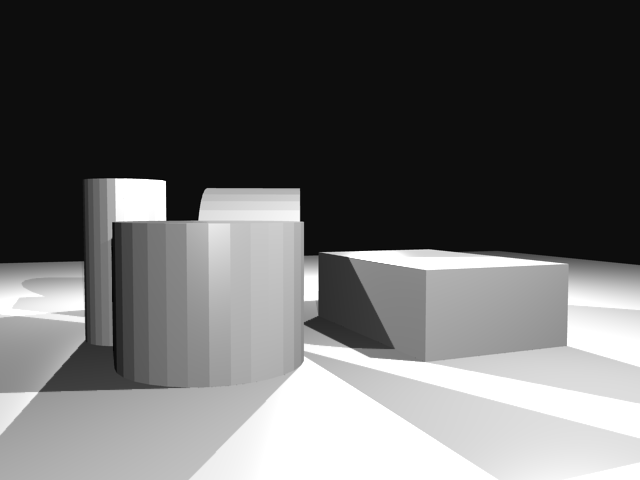
\includegraphics[height=\turnheight]{umk4nke6pzebef2b_SEQ_input.png} &
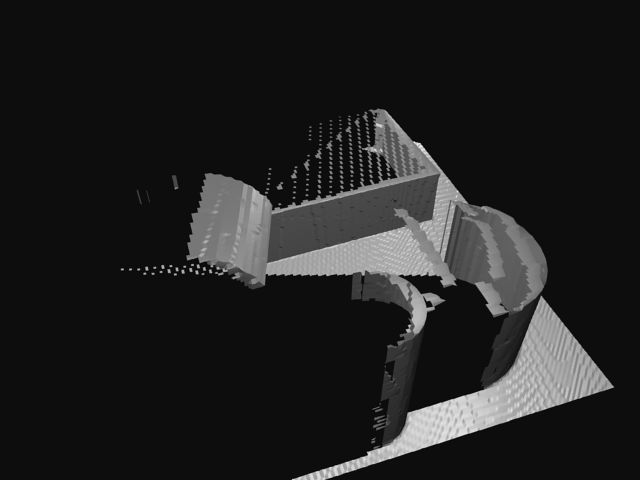
\includegraphics[height=\turnheight]{umk4nke6pzebef2b_SEQ_visible.png} &
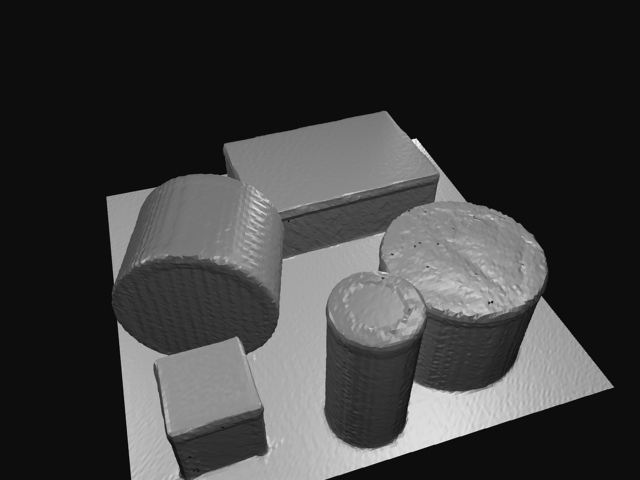
\includegraphics[height=\turnheight]{umk4nke6pzebef2b_SEQ_gt.png} &
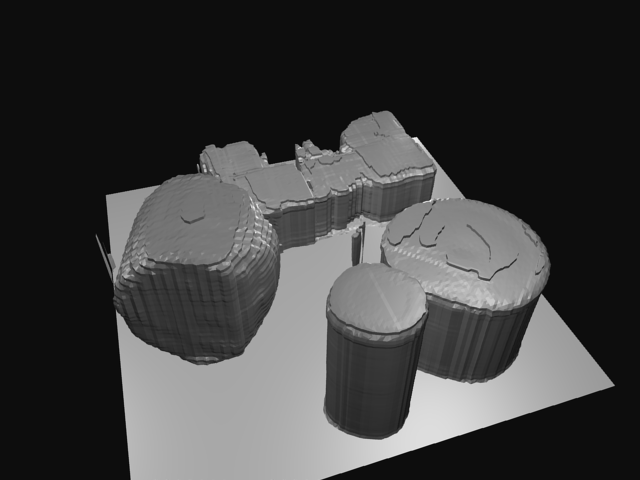
\includegraphics[height=\turnheight]{umk4nke6pzebef2b_SEQ_pred_voxlets.png} \\
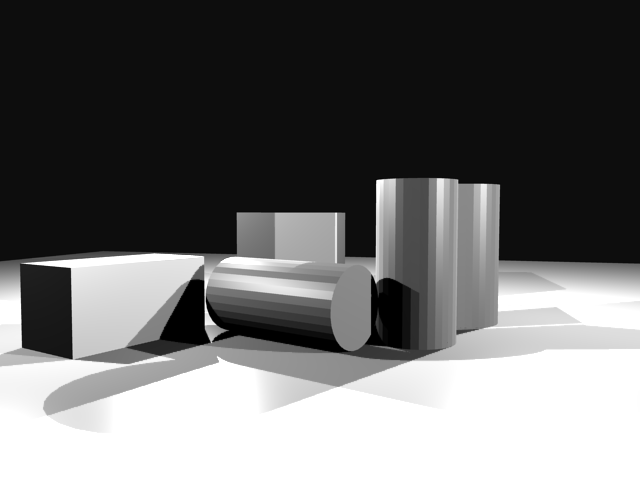
\includegraphics[height=\turnheight]{xf2hcoes8lp9fb1t_SEQ_input.png} &
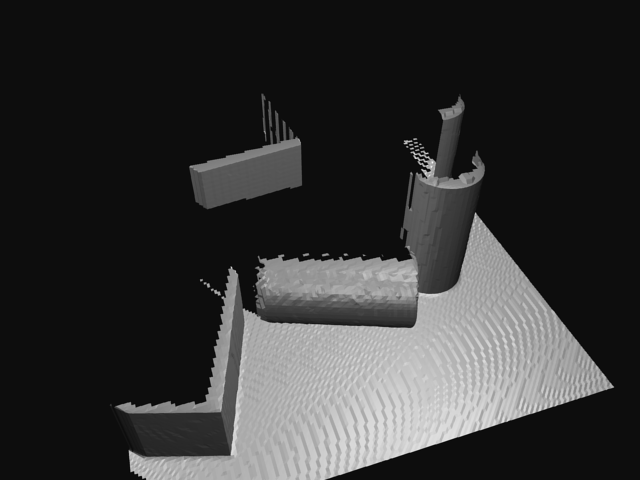
\includegraphics[height=\turnheight]{xf2hcoes8lp9fb1t_SEQ_visible.png} &
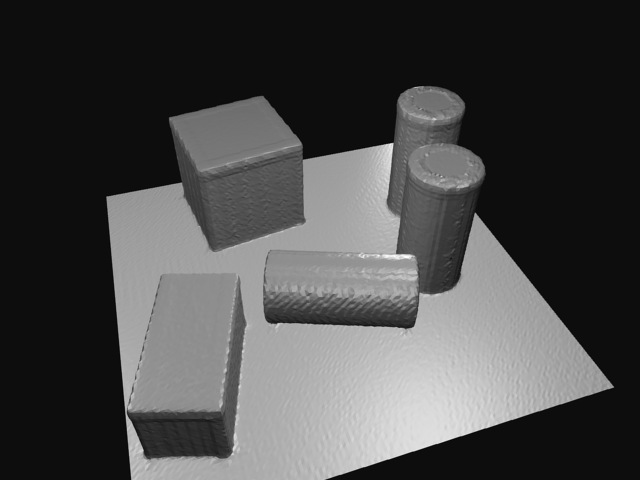
\includegraphics[height=\turnheight]{xf2hcoes8lp9fb1t_SEQ_gt.png} &
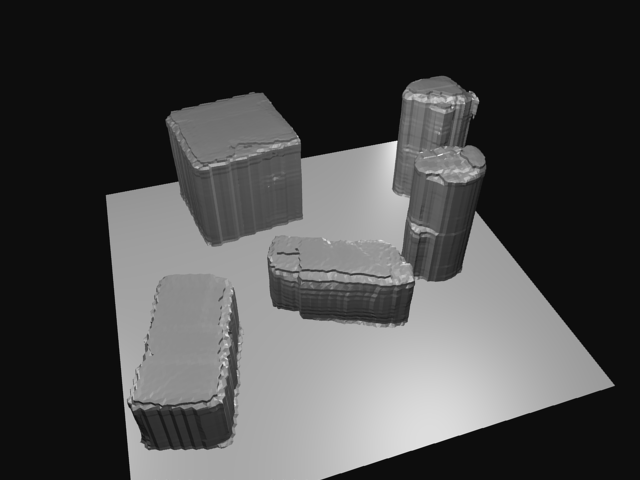
\includegraphics[height=\turnheight]{xf2hcoes8lp9fb1t_SEQ_pred_voxlets.png} \\
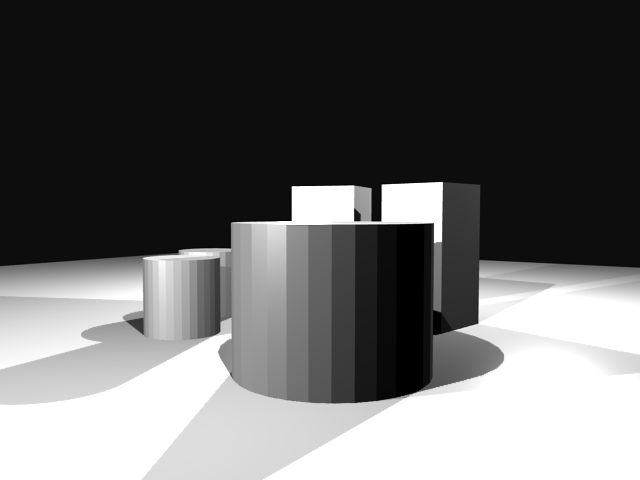
\includegraphics[height=\turnheight]{kmrkmma8u2456lgk_SEQ_input.png} &
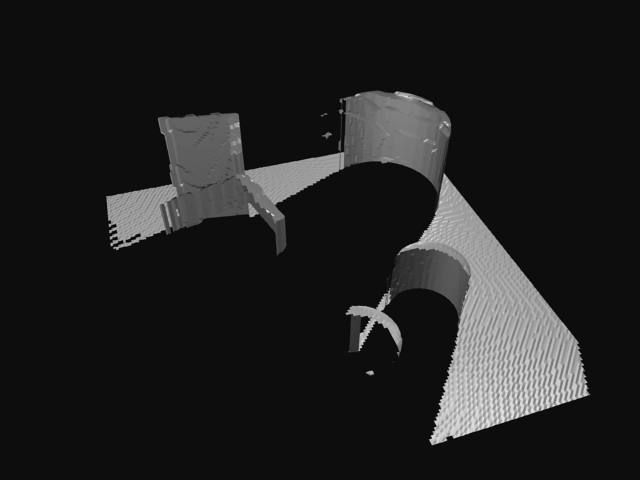
\includegraphics[height=\turnheight]{kmrkmma8u2456lgk_SEQ_visible.png} &
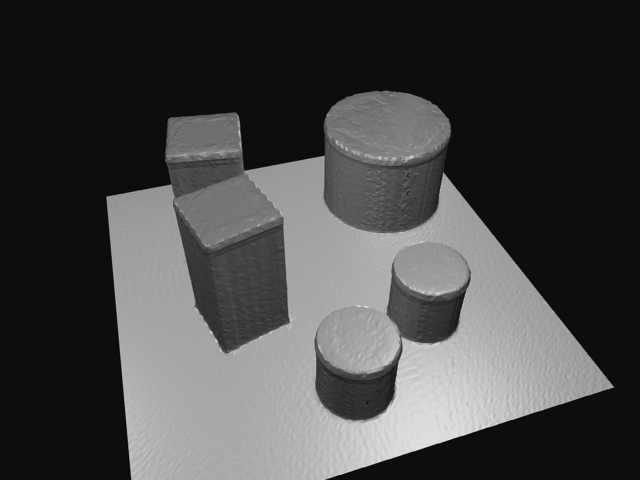
\includegraphics[height=\turnheight]{kmrkmma8u2456lgk_SEQ_gt.png} &
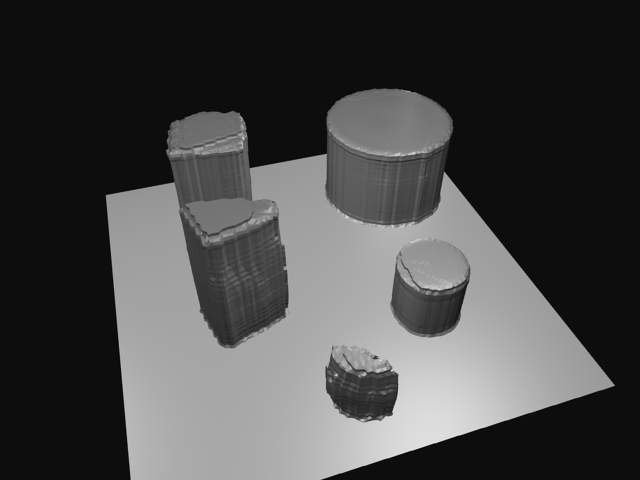
\includegraphics[height=\turnheight]{kmrkmma8u2456lgk_SEQ_pred_voxlets.png} \\
\footnotesize Input view of scene &
\footnotesize Input data in 3D space &
\footnotesize Ground truth occupancy &
\footnotesize Our reconstruction \
\end{tabular}
\end{figure*}

    \vspace{2pt}
     \caption{
     Qualitative results from our synthetic scene dataset.
     Each row shows a different configuration of synthetic objects.
     We note that, compared to Forest Medoid, {\bf Voxlets} successfully recovers the shape of many objects.
     It is in areas of occlusions, and heavy clutter (row three) that are the most difficult to complete.
     }
     \label{fig:synth_results}
\end{figure*}


We can gain some insight into the performance of {\bf Voxlets} by replacing various stages with an oracle that has access to the ground truth:

\noindent\textbf{V}$_\text{gt}$: Instead of using the structured prediction, the ground truth voxels are extracted and then placed directly into the output grid. This baseline embodies the best output that a perfectly-trained version of our model could produce. %evaluates how good the space of voxlets is.

\noindent\textbf{V}$_\text{pca}$: The ground truth voxlets are compressed, then decompressed, using a pre-learned PCA model. This baseline evaluates how well PCA covers the range of voxlet shapes.

\noindent\textbf{V}$_\text{nn}$: We find a nearest neighbor training example for the ground truth voxlet at each location. These are the best possible predictions, given this training set. %The predictions are still restricted to be training examples.

\noindent\textbf{V}$_\text{agg}$: We use our structured Random Forest algorithm for prediction with the oracle at the aggregation step. Each voxlet is greedily added to the accumulator only if its inclusion increases the score for the given scene.

Results for these different configurations are presented in Table \ref{tab:oracle_results}.

\begin{table}
  \centering
  \begin{tabular}{|p{2.2cm}|c|c|c|c|}
  \hline
  \textbf{Method}  &   \textbf{Precision} & \textbf{Recall} & \textbf{IoU}\\
  \hline
   \textbf{V}$_\text{gt}$ & {\bf 0.958} & {\bf 0.903} & {\bf 0.866} \\
  \textbf{V}$_\text{pca}$ & 0.954  & 0.898 & 0.864 \\
  \textbf{V}$_\text{nn}$ & {\bf 0.958} & 0.845 & 0.815 \\
  \textbf{V}$_\text{agg}$ & 0.939 & 0.860 & 0.815 \\
  \hline
  {\bf Voxlets} & 0.864 & 0.833 & 0.737 \\
  \hline
  \end{tabular}
  \vspace{5pt}
  \caption{Quantitative results of different oracle-enhanced versions of {\bf Voxlets} on our synthetic dataset. Dimensionality reduction hurts the scores very little. The nearest neighbor scores suggest that the training data contains unexploited variety. Better aggregation of voxlets could better exploit the forest's predictions.}
  \vspace{-5pt}
    \label{tab:oracle_results}
\end{table}


%%%%%%%%%%%%%%%%%%%%%%%%%%%%%%%%%%%%%%%%%%%%
\subsection{Tabletop scenes}
\label{sec:exp_tt}
Here we perform experiments on our real tabletop dataset, introduced in Section~\ref{sec:datasets}.
Results are presented in Figures~\ref{fig:tabletop_res} and~\ref{fig:intro}. Results are noteworthy because so many missing voxels in the input scan are correctly filled in, despite severe occlusions and fragmentation of objects. For more results, please see our supplementary files.

\begin{figure*}[!t]
    \newcommand{\turnheight}{0.23\columnwidth}
\begin{figure*}
\begin{tabular}{cccc}
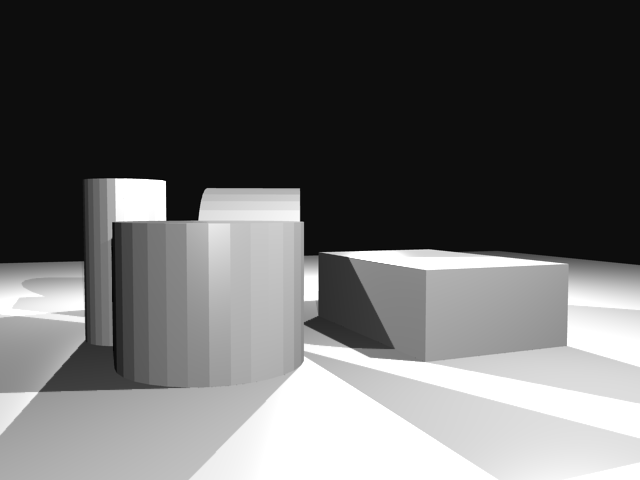
\includegraphics[height=\turnheight]{umk4nke6pzebef2b_SEQ_input.png} &
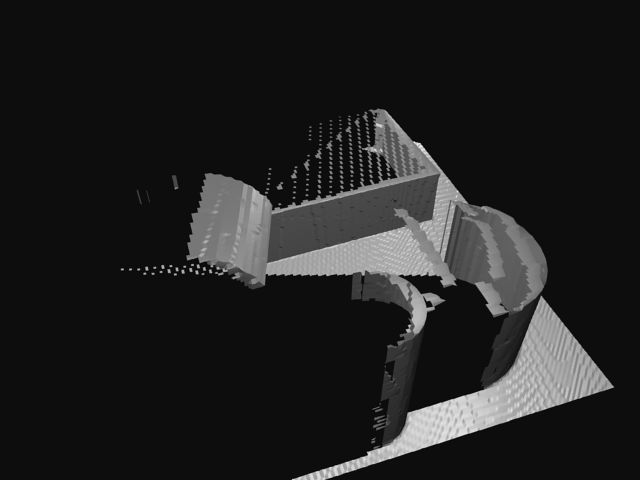
\includegraphics[height=\turnheight]{umk4nke6pzebef2b_SEQ_visible.png} &
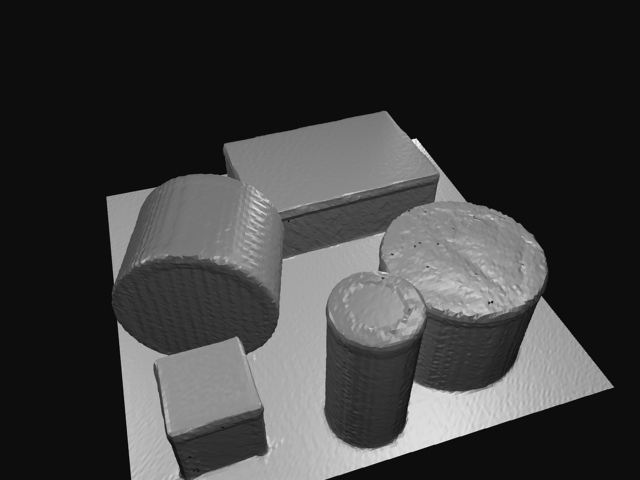
\includegraphics[height=\turnheight]{umk4nke6pzebef2b_SEQ_gt.png} &
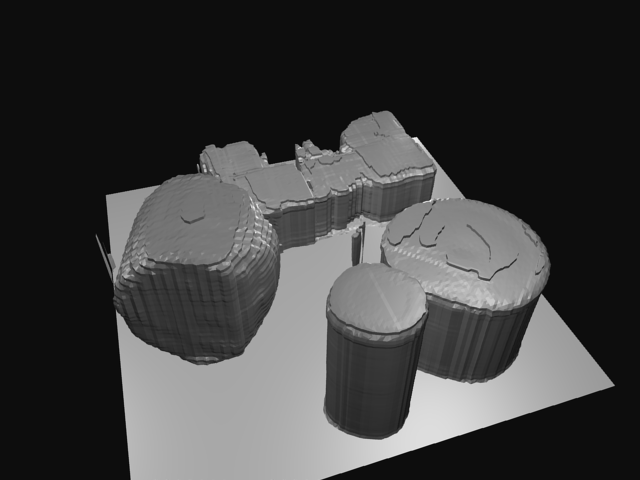
\includegraphics[height=\turnheight]{umk4nke6pzebef2b_SEQ_pred_voxlets.png} \\
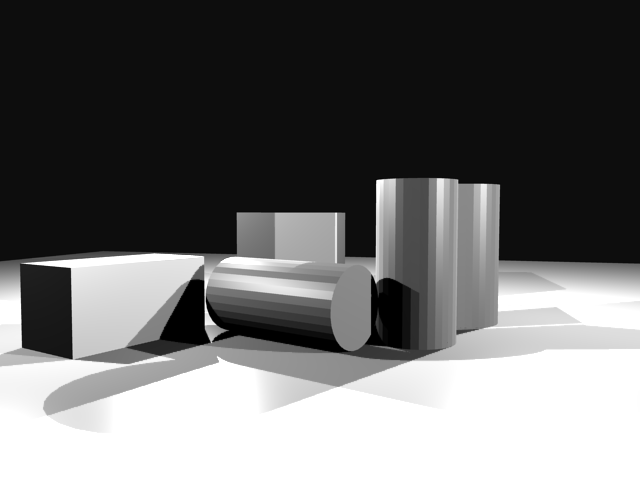
\includegraphics[height=\turnheight]{xf2hcoes8lp9fb1t_SEQ_input.png} &
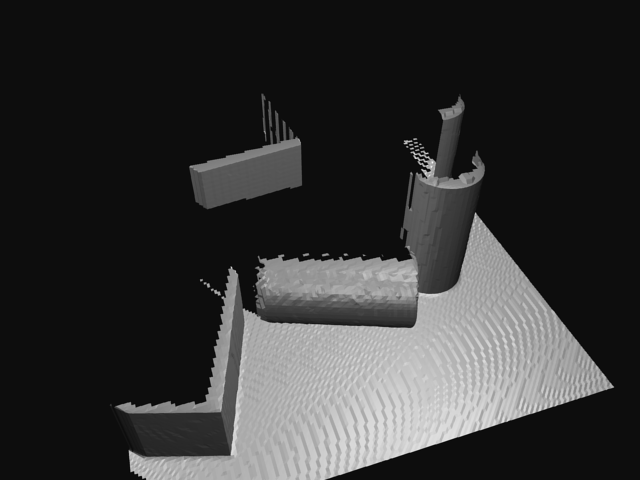
\includegraphics[height=\turnheight]{xf2hcoes8lp9fb1t_SEQ_visible.png} &
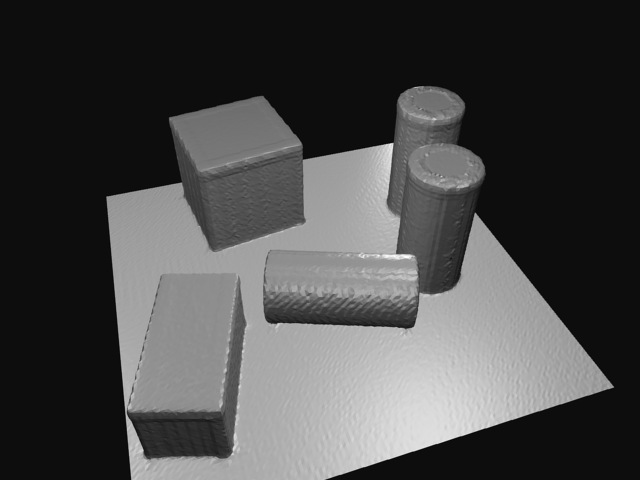
\includegraphics[height=\turnheight]{xf2hcoes8lp9fb1t_SEQ_gt.png} &
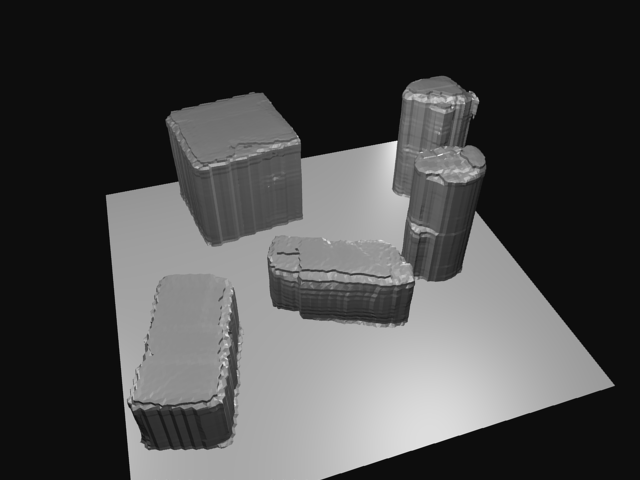
\includegraphics[height=\turnheight]{xf2hcoes8lp9fb1t_SEQ_pred_voxlets.png} \\
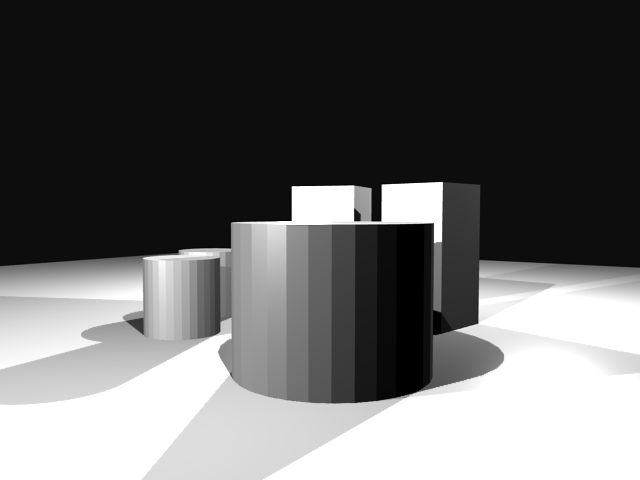
\includegraphics[height=\turnheight]{kmrkmma8u2456lgk_SEQ_input.png} &
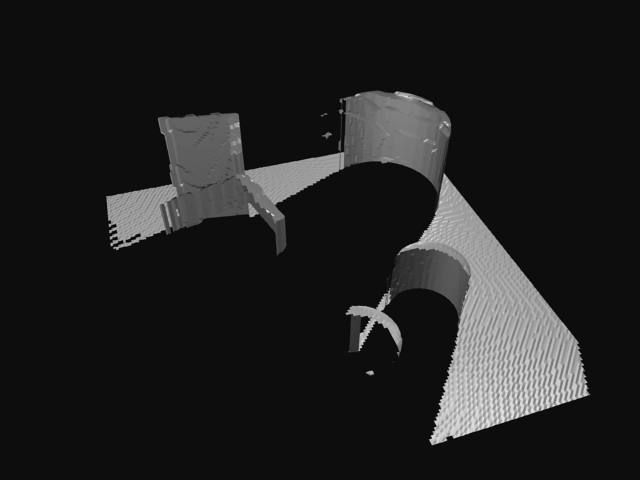
\includegraphics[height=\turnheight]{kmrkmma8u2456lgk_SEQ_visible.png} &
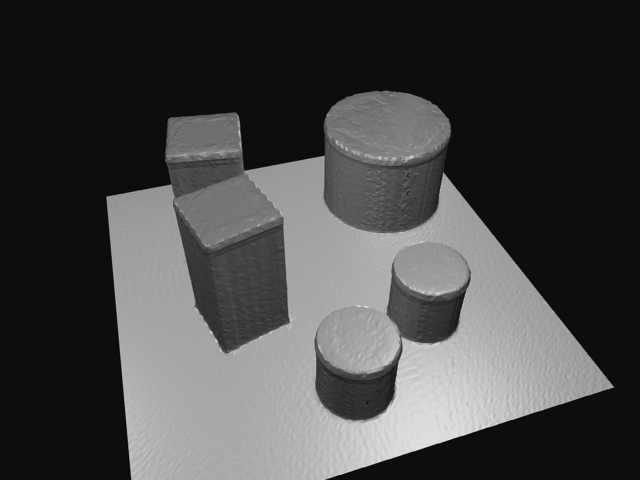
\includegraphics[height=\turnheight]{kmrkmma8u2456lgk_SEQ_gt.png} &
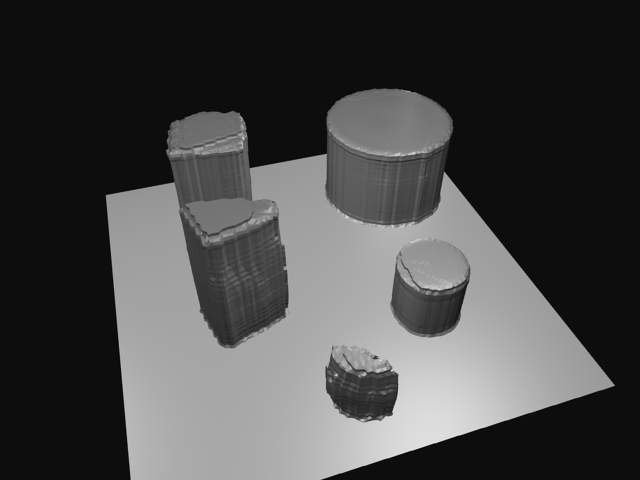
\includegraphics[height=\turnheight]{kmrkmma8u2456lgk_SEQ_pred_voxlets.png} \\
\footnotesize Input view of scene &
\footnotesize Input data in 3D space &
\footnotesize Ground truth occupancy &
\footnotesize Our reconstruction \
\end{tabular}
\end{figure*}

    \vspace{5pt}
     \caption{
     Results for our tabletop dataset using data captured with a Kinect, where the input camera view is indicated by a black arrow.
     For clarity, we insert a ground plane during rendering and do not superimpose the observed input geometry on top of our predictions.
     The kettle's handle in row three highlights an interesting failure case, where no  similar objects are present in the training data.
     {\bf Voxlets} still succeeds in capturing the coarse geometry of the object.
     }
     \label{fig:tabletop_res}
\end{figure*}

In Table~\ref{tab:tabletop_tab}, we evaluate the three alternative strategies for interpreting predictions from our structured forest, as described in Section~\ref{sec:agg_predictions}.
We can see that our `Observed Fit' approach is better overall than other baselines, with very good recall and IoU.
As a result of multiple conflicting overlapping predictions, `Forest Medoid' and `Forest Mean' tend to underpredict, resulting in higher precision but poorer recall and IoU (see Figure~\ref{fig:tabletop_res}).
We favor 'Observed Fit' because it chooses the prediction that agrees most with the observed geometry at each sample point, resulting in better completions.
% `Forest Medoid' and `Forest Mean' tend to underpredict, resulting in better precision but poorer recall and IoU (see Figure~\ref{fig:tabletop_res} for an example).

\begin{table}
  \centering
  \begin{tabular}{|p{2.5cm}|c|c|c|}
  \hline
  \textbf{Method}  &   \textbf{Precision} & \textbf{Recall} & \textbf{IoU}\\
  \hline
    Forest Mean  & {\bf 0.941} &  0.240 & 0.236 \\
    Forest Medoid & 0.935 &  0.286 &     0.279 \\
    {\bf Observed Fit}  & { 0.883} & {\bf 0.684} & {\bf 0.625} \\
  \hline
  \end{tabular}
  \vspace{5pt}
  \caption{Quantitative results for the tabletop dataset,  comparing different prediction selection strategies.}
    \label{tab:tabletop_tab}
    \vspace{-5pt}
\end{table}

%%%%%%%%%%%%%%%%%%%%%%%%%%%%%%%%%%%%%%%%%%%%
\subsection{Qualitative scene results}
Finally, in Figure~\ref{fig:nyu_results}, we present results on depth images from NYU-Depth V2 \cite{silberman-eccv-2012}, using our model from the tabletop training set.
We assume the largest horizontal plane has been extracted from the scene, and the voxel grid is placed on top of that plane.
Here we extract the plane manually, but this could be achieved automatically~\eg \cite{silberman-eccv-2012}.
Predicting the occupancy for a single scene takes less than 30 seconds using our unoptimized Python implementation.


\begin{figure}
    \vspace{-10pt}
  \includegraphics[width=0.8\columnwidth]{nyu}
         \caption{Our occupancy predictions for two scenes from the NYU-Depth V2 dataset \cite{silberman-eccv-2012}. On the left, we are able to successfully recover the geometry of the scene, even with very sparse and noisy input depth.
On the right, the input depth provides no cues as to the shape of the desktop PCs, so the predictions are too shallow.}%
    \label{fig:nyu_results}
        \vspace{-12pt}
\end{figure}



%%%%%%%%%%%%%%%%%%%%%%%%%%%%%%%%%%%%%%%%%%%%
% \note{OMA: Point to specific places in results to show limitations, maybe NYU?}
\paragraph{Limitations}\newline
Sharp edges are frequently rounded due to averaging. Also, as a supervised learning algorithm, {\bf Voxlets} is limited by the data available at training time.
This can be seen in Figure~\ref{fig:nyu_results}, as no computer-sized objects are in the training set.
Currently, our voxlets are a fixed size, and success correlates with the test-scene having similar sized objects.
% In our work we use two sizes of voxlet, but

%We can see that while we have success reconstructing well-observed objects, our algorithm can fail to recover geometry in occluded regions.
%Furthermore, by training on real-world scenes wo
% There are

%%%%%%%%%%%%%%%%%%%%%%%%%%%%%%%%%%%%%%%%%%%%
\section{Conclusions and future work}
We have demonstrated that {\bf Voxlets} successfully recover 3D geometry from only a single input depth image. Our algorithm efficiently combines both shape selection and pose estimation, using simple feature test evaluations to predict local geometry occupancy.
Voxlets are learned from training data, which has so far included only man-made table-top sized objects. Even similar objects vary in size and viewing direction, but objects from distinct semantic classes share enough 3D shape components to allow good, though not perfect, reconstructions.

For some applications, the quality of our predictions may already be enough, \eg to aid robot grasping or navigation. Currently, there is nothing guaranteeing that our results are physically stable or smooth.
How to best incorporate physics-based reasoning~\cite{zheng-cvpr-2013, shao-siggraphasia-2014} is still an open problem, but enforcing this strong prior may improve accuracy. %result in even more accurate results.
One interesting potential application of our method is to use the predicted completion as a prior for SLAM.
As new data arrives, a next-best-view algorithm~\cite{Potthast2014148} could leverage our predictions.

%Currently we use a random sampling strategy to select the set of 3D points to use to form the reconstruction.
%We believe that a more intelligent sampling strategy, such as using the points which we believe to give accurate estimates of the depth \cite{reynolds-cvpr-2011}, may yield more accurate reconstructions.
%We would like to incorporate ideas from \cite{zheng-cvpr-2013, shao-siggraphasia-2014} by incorporating physics-based reasoning to help the completion of ambiguous regions.
%We also believe a coarse-to-fine version of our system would help to make the method more robust.



% \section{Acknowledgements}
% Peter Gehler
% Malcolm
% Neill
% Prism group
% Tom
% Peter
% Yotam
% JJ
% Open source community - python scipy pcl etc

\pagebreak
{\fontsize{9}{10}\selectfont
\bibliographystyle{ieee}
\bibliography{bibtex/strings.bib,bibtex/main.bib}
}


\end{document}